\documentclass[a4paper,12pt]{article} %style de document
\usepackage[utf8]{inputenc} %encodage des caractères
\usepackage[french]{babel} %paquet de langue français
\usepackage[T1]{fontenc} %encodage de la police
\usepackage[top=2cm,bottom=2cm,left=2cm,right=2cm]{geometry} %marges
\usepackage{graphicx} %affichage des images
\usepackage{amssymb}
\usepackage{url}
\usepackage{verbatim}
\usepackage{amsmath}

\begin{document} %début du document



%----------------------------------
%page de garde
%----------------------------------

\begin{titlepage}

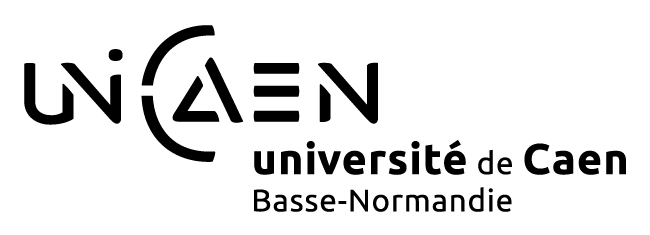
\includegraphics[scale=0.3]{images/unicaen.png}

\vspace{7cm}

\begin{center}

\begin{Huge}
Sécurité et Aide à la Décision\\
Expérimentations du TP\\
\end{Huge}
\vspace{2cm}
\begin{large}
Mori Baptiste 21602052\\
Leblond Valentin 21609038\\
\vspace{1cm}
L2-Info-groupe-4A
\end{large}

\end{center}
\end{titlepage}


%------------------------------
%sommaire
%------------------------------

\newpage

\tableofcontents{}

\newpage

%------------------------------
%contenu
%------------------------------


\section*{Introduction}
\addcontentsline{toc}{section}{Introduction}

L'objectif de ce TP est de mettre en place deux intelligence artificielles, la première fonctionnant avec l'algorithme Minmax et l'autre avec l'algorithme Alphabeta. Ces intelligences artificielles nous servirons à choisir le meilleurs coup à jouer sur une profondeur donnée.

Nous allons procéder à des expérimentation sur le nombre de nœuds que parcours chaque algorithme afin de comparer Minmax et Alphabeta.

\section{Désaccord sur les choix des deux algorithmes}

Nous avons mis les deux algorithme en parallèle sur le même réseaux pour voir si ils avaient les mêmes décisions de coups. Nous avons remarqué que, pour le cas de l'attaque, il arrivait qu'ils soient en désaccord. Comme on peut le voir sur la capture ci-dessous dans l'état actuel Alphabeta choisi d'infecter l'ordinateur 2 alors que Minmax choisi l'ordinateur 3.

\begin{center}
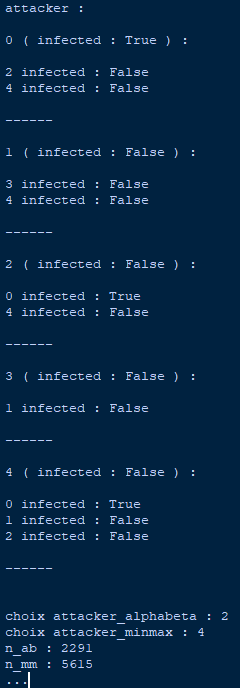
\includegraphics[scale=0.7]{images/Capture2.PNG}
\end{center}

Les deux algorithmes mènes à deux états finaux différents, pour Alphabeta on a le défenseur qui gagne et pour Minmax c'est l'attaquant qui gagne. Les défenseurs ont également des valeurs différentes, plus importante chez Alphabeta mais la valeur des défenseurs étant différente ne nous dis rien sur le faite que l'un est plus efficace que l'autre car on fait jouer un attaquant Alphabeta contre un défenseur Alphabeta de même pour Minmax.

\begin{center}
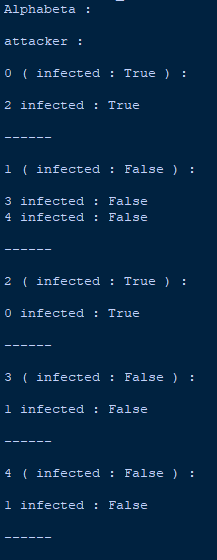
\includegraphics[scale=0.7]{images/Capture3.PNG}
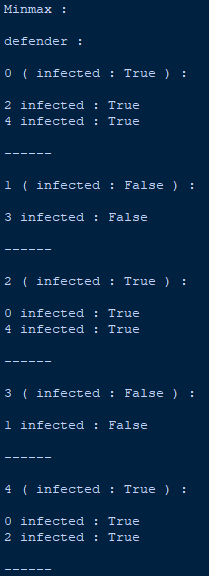
\includegraphics[scale=0.7]{images/Capture4.PNG}\\
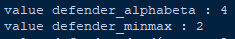
\includegraphics[scale=1]{images/Capture5.PNG}
\end{center}

Nous nous avons donc pensé que Alphabeta favorisé le défenseur et Minmax l'attaquant, nous avons donc tester de faire jouer un Alphabeta attaquant contre un Minmax défenseur et un Minmax attaquant contre un Alphabeta défenseur sur la même génération de graph (étant donnée qu'ils jouent quasiment la même chose on a lancé plusieurs fois le jeu afin de tomber sur un désaccord).

\begin{center}
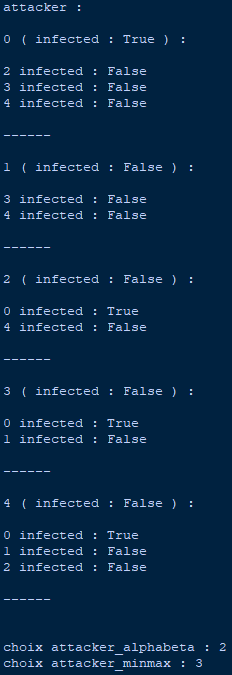
\includegraphics[scale=0.7]{images/Capture6.PNG}
\end{center}

Sur les résultats finaux des deux batailles, on remarque que quand Alphabeta attaque (capture de gauche), il gagne quand même mais il a infecté que 3 ordinateurs sur 5 et quand Minmax attaque (capture de droite) il en a infecté 4 sur 5.

\begin{center}
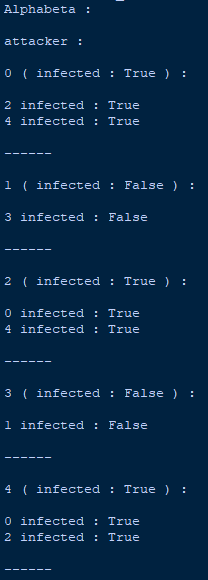
\includegraphics[scale=0.7]{images/Capture7.PNG}
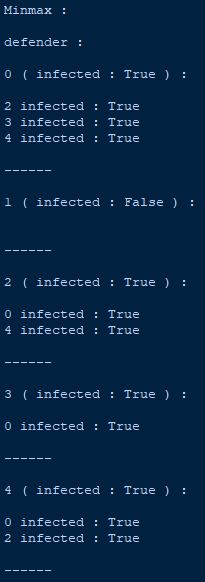
\includegraphics[scale=0.7]{images/Capture8.PNG}\\
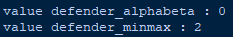
\includegraphics[scale=1]{images/Capture9.PNG}
\end{center}

Malgré ces testes, nous ne pouvons rien dire sur l'efficacité des ses deux algorithme qui semblent presque équivalent en terme de résultat.

\section{Tests sur le nombre de parcours des nœuds}

Nous allons nous intéresser à comparer le nombre de nœuds que parcourt chaque algorithme. Pour cela, nous avons implémenté un compteur dans le constructeur de la classe de L'IA afin de compter chaque passage dans Minmax et dans Alphabeta.\\

Dans un premier temps, nous allons faire varier le nombre de profondeur auquel les algorithme vont regarder tout en gardant le même graph de départ pour le test de chaque profondeur. Nous utiliseront Matplotlib et Numpy pour construire nos graphiques.

\begin{center}
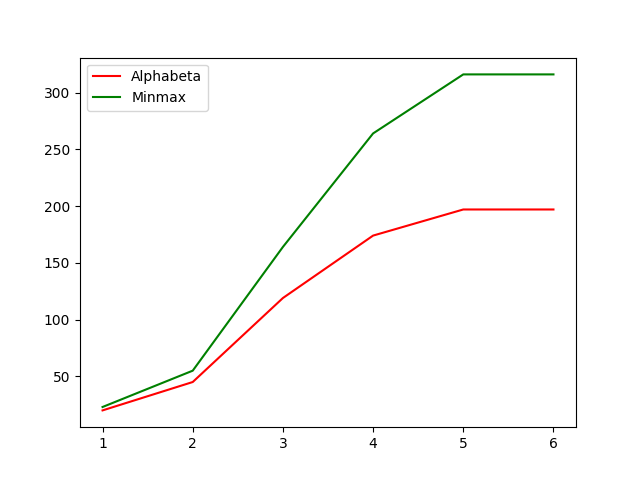
\includegraphics[scale=0.5]{images/Figure_1.png}
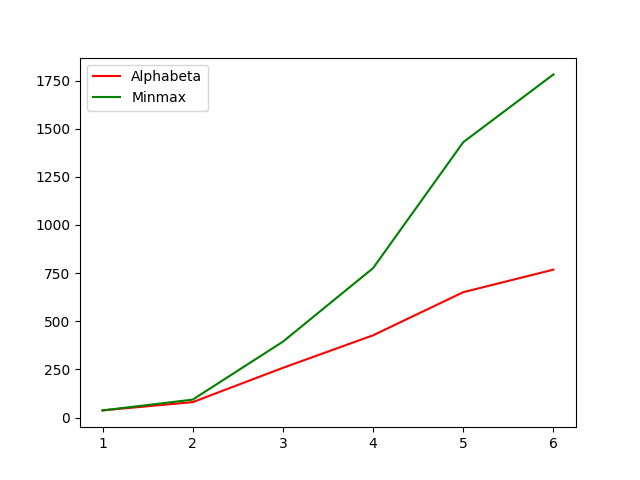
\includegraphics[scale=0.5]{images/Figure_2.png}
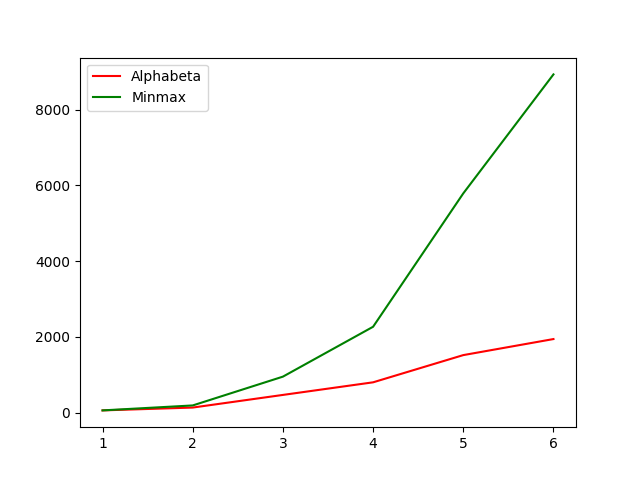
\includegraphics[scale=0.5]{images/Figure_3.png}\\
Nombre de nœuds parcourus en fonction de la profondeur
\end{center}

On remarque que pour chaque test, Alphabeta est toujours bien en dessous en terme de parcours que Minmax, même si pour le premier graphique le graph du jeu semble un peux particulier (le passage entre la profondeur 5 et 6 n'a pas changer énormément le nombre de parcours), Alphabeta semble parcourir le moins de nœuds quelque soit la profondeur qu'on lui donne.\\

Dans un second temps, nous allons faire varier la probabilité que deux ordinateurs soient connectés (cette fois nous recréons à chaque fois un nouveau graph d'où les courbes un peu chaotique).

\begin{center}
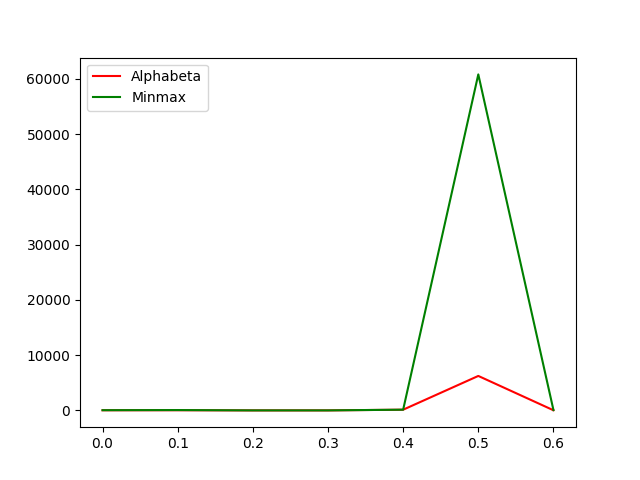
\includegraphics[scale=0.5]{images/Figure_4.png}
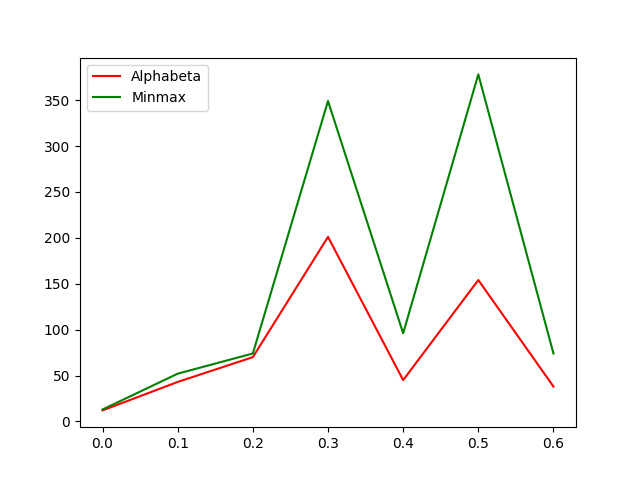
\includegraphics[scale=0.5]{images/Figure_5.png}
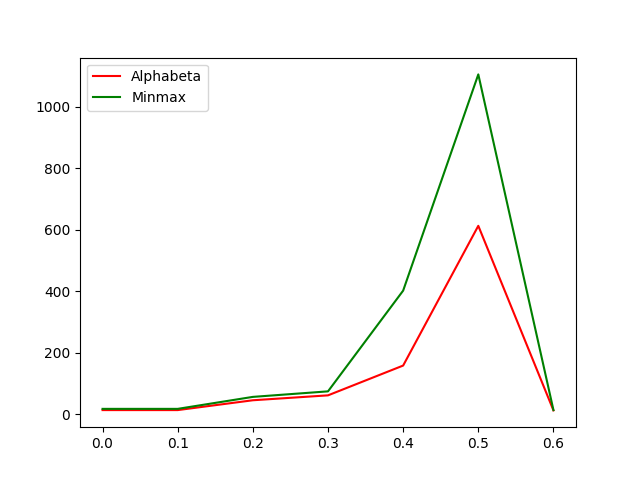
\includegraphics[scale=0.5]{images/Figure_6.png}\\
Nombre de nœuds parcourus en fonction de la probabilité
\end{center}

On remarque de même que Alphabeta parcours moins de nœuds que Minmax et que plus Minmax parcours de nœuds, plus l'écart entre les deux est important, il y a donc une relation de puissance sur le nombre de nœuds parcourus par ces deux algorithmes.

\section*{Conclusion}
\addcontentsline{toc}{section}{Conclusion}

Alphabeta et Minmax ayant quasiment les mêmes décisions sur les coups à jouer, Alphabeta est celui qui parcours le moins de nœuds et donc qui est le plus rapide dans sa prise de décision.

\end{document}
